%+----------------------------------------------------------------------------+
%| SLIDES:  short talk WORKSHOP ON MULTISYMPLECTIC GEOMETRY
%| Url: [https://wis.kuleuven.be/events/multisymplectic]
%| Contents: 9 Technical Slides  
%|					 (extimated duration 3 minutes per slide )
%| Author: Antonio miti
%| Place: Online (Zoom), September 2020
%+----------------------------------------------------------------------------+


%- HandOut Flag -----------------------------------------------------------------------------------------
\newif\ifHandout
	\Handouttrue  %uncomment for the printable version


%- D0cum3nt ----------------------------------------------------------------------------------------------
\ifHandout
	\documentclass[handout,10pt]{beamer}   
	\setbeameroption{show notes} %print notes    
\else
	\documentclass[10pt]{beamer}
\fi


%- Packages ----------------------------------------------------------------------------------------------
\usepackage{verbatim}
\usepackage{appendixnumberbeamer}
\usepackage[mode=buildnew,subpreambles=true]{standalone}
\usepackage{amsmath, amssymb}
\usepackage{tikz}
\usetikzlibrary{decorations.pathmorphing}
\usetikzlibrary{arrows,shapes,calc}
\usepackage{tikz-cd}
\usepackage{graphicx, animate}
\usepackage{hyperref}
\usepackage[english]{babel}
\usepackage{csquotes}
\usepackage{wasysym}
%\usepackage{enumitem} %option in itemize
\usepackage{xcolor}
\usepackage{pifont}
\usepackage{empheq}
\usepackage[font=scriptsize]{caption}
\usepackage{cancel}

\usepackage[cal=boondox,scr=boondoxo]{mathalfa}
% use mathscr for the v denoting hamiltonian vector fields. Avoid confusion with the infinitesimal action v!


\newcommand{\cmark}{\textcolor{green}{\ding{51}}}%
\newcommand{\xmark}{\textcolor{red}{\ding{55}}}%



%--Beamer Style-----------------------------------------------------------------------------------------------
\usetheme{toninus}

%- T1tle P4g3 -------------------------------------------------------------------------------------------
\title{Homotopy co-moment maps for compact actions on spheres} 
\author[AMM]{\href{https://dmf.unicatt.it/miti/}{Antonio Michele Miti}
	\\
	(Joint work with Leonid Ryvkin)
}
\subtitle{Based on \href{https://arxiv.org/abs/1906.08790}{arXiv:1906.08790}}
\institute[UCSC and KU Leuven]{
  \begin{tabular}[h]{ccc}
      Università Cattolica del Sacro Cuore & \qquad\qquad & KU Leuven \\
      Brescia, Italy & & Leuven, Belgium \\
      \href{https://dipartimenti.unicatt.it/dmf-home?rdeLocaleAttr=it}{
\includegraphics[width=3.5cm]{Logos/UnicattBS-logo}} & & 
      \href{https://wis.kuleuven.be/english}{
\includegraphics[width=4cm]{Logos/KULeuven_logo}}
  \end{tabular}      
}
\date[KULeuven_20] % (optional, should be abbreviation of conference name)
{	
	\href{https://wis.kuleuven.be/events/multisymplectic}{Online workshop on Multisymplectic Geometry} \\
	{\vskip 1ex}
	Leuven, September 10, 2020
}


%- WorkAround --------------------------------------------------------------------------------------------------------------
%Standalone with relative path
\newcommand{\includestandalonewithpath}[3][]
{
  \begingroup
  \newcommand{\datapath}{#2}
  \includestandalone[#1]{\datapath/#3}
  \endgroup
}

%Intermediate checkpoint slide
\newcommand{\checkpoint}[0]{
	\ifHandout

	\else
	\addtocounter{framenumber}{-1}
 	\begin{frame}{Outline}
  		%\tableofcontents[currentsection,currentsubsection]
  		\tableofcontents[currentsection]
	\end{frame}
	\fi
}
%
\newcommand{\outline}[0]{
	\ifHandout

	\else
	\addtocounter{framenumber}{-1}
 	\begin{frame}{Outline}
  		%\tableofcontents[currentsection,currentsubsection]
  		\tableofcontents
	\end{frame}
	\fi
}
%
\newcommand{\thankyouslide}[0]{
	\ifHandout

	\else
	\addtocounter{framenumber}{-1}
	\begin{frame}{}
		\vfill
	  \centering 
	  {\Huge\color{red} 
	  \emph{Thank you for your attention!}}
		\vfill
		%
		\centering
		\begin{columns}
			\hfill
			\begin{column}{0.05\linewidth}
				\centering \includegraphics{beamericonarticle}
			\end{column}
			\begin{column}{0.8\linewidth}
				\centering
				\textbf{Multisymplectic actions of compact Lie groups on spheres},
				\\
				\href{a}{arXiv:1906.08790} (to appear on \emph{Journal of Symplectic Geometry}),
				\\
				\emph{AMM, Leonid Ryvkin}.
			\end{column}
			\begin{column}{0.05\linewidth}
				\centering \includegraphics{beamericonarticle}			
			\end{column}
			\hfill
		\end{columns}
		\vfill		  
	\end{frame}
	\fi
}






%---------------------------------------------------------------------------------------------------------------------------------------------------
%- D0cum3nt ----------------------------------------------------------------------------------------------------------------------------------
\begin{document}
\addtocounter{framenumber}{-1}

%-------------------------------------------------------------------------------------------------------------------------------------------------
	\begin{frame}  % Alternative: \maketitle outside of frame
	  \titlepage
	  \ifHandout
		  \tikz[overlay,remember picture]
			{
	    		%	\node at ($(current page.west)+(1.5,0)$) [rotate=90] {\Huge\textcolor{gray}{\today}};
	    			\node[        draw,
	        			shape border rotate=90,
					isosceles triangle,
			        isosceles triangle apex angle=90,
	        			fill=yellow]
	        		at ($(current page.north east)-(1,1)$) [rotate=-45] {\textcolor{red}{Annoted version}};
			}
	\fi
	\end{frame}
	\note{
		\scriptsize{
		\textbf{\underline{Abstract:}}\\
			Five years ago, Callies, Fregier, Rogers, and Zambon, introduced a natural extension of the notion of comoment map to the context of multisymplectic geometry. 
			They call \emph{Homotopy comoment map} an $L_{\infty}$ morphism associated with certain infinitesimal actions which preserve the multisymplectic form of a target manifold. 
			Being this concept particularly subtle and technical, there are not so many meaningful examples worked out in full details.
			In this talk, we try to address this problem by giving new insights on multisymplectic actions of compact groups and thus deriving existence results and explicit constructions for comoment maps related to actions on spheres.
			Namely, we will discuss the existence problem for compact effective group actions on spheres and provide explicit constructions for such homotopy comoment maps in particular cases.
			\\
			This is joint work with Leonid Ryvkin.

			\vspace{1em}
			\textbf{\underline{Outline:}}\\
			\vspace{-1em}
	  		\tableofcontents		
			}
	}
%---------------------------------------------------------------------------------------------------------------------------------------------------
%---------------------------------------------------------------------------------------------------------------------------------------------------
\outline

%-------------------------------------------------------------------------------------------------------------------------------------------------
%-------------------------------------------------------------------------------------------------------------------------------------------------
\section{Background}
%\checkpoint
%-------------------------------------------------------------------------------------------------------------------------------------------------
\subsection{Symplectic geometry}
\begin{frame}{Reminder: Symplectic geometry}
\begin{columns}[T]
	\begin{column}{.50\linewidth}
		\minipage[c][0.9\textheight][s]{\columnwidth}
		% workaround: why does vfill not work inside beamer column?
		\begin{defblock}[Symplectic Manifold]
			\vspace{-1em}
			\includestandalone[width=\textwidth]{Pictures/Figure_sym}	
		\end{defblock}
		%
		\pause
		\begin{exblock}[$M = T^\ast Q$ is symplectic]
			$\omega = d \theta $ with
			$$ \left.\theta\right\vert_{(q,p)} (v) = p (\pi_\ast v) ~.$$
		\end{exblock}
		%
		\begin{columns}
			\begin{column}{.50\linewidth}
				\begin{center}
					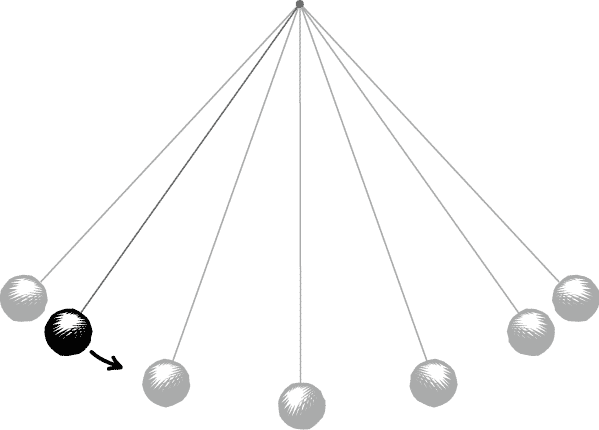
\includegraphics[width=0.8\linewidth]{Pictures/pendulum13}			
				\end{center}
			\end{column}	
			\begin{column}{.50\linewidth}
				\begin{center}
					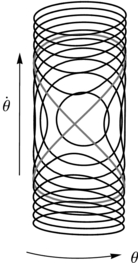
\includegraphics[width=0.45\linewidth]{Pictures/pendulum-phase-space}			
				\end{center}
			\end{column}	
		\end{columns}
		%
		\vfill
		\centering
		\textit{ "geometric approach" to mechanics \dots}
		%
		\endminipage
	\end{column}
	\vrule{}
	\pause
	\begin{column}{.50\linewidth}
		\minipage[c][0.9\textheight][s]{\columnwidth}
		%
		\begin{defblock}[Classical Observables]
			Unital, associative, commutative algebra $C^\infty(M)$.
		\end{defblock}
		%
		\vfill
		\pause
		\begin{defblock}[Hamiltonian vector fields]
			$\mathscr{v}_f \in \mathfrak{X}(M)$ such that:
			$$\iota_{\mathscr{v}_f} \omega = -df \quad \text{(exact)}$$ %$\in B^1(M)$
			\small$\mathscr{v}_f$ = \emph{Ham.v.f. pertaining to $f\in C^\infty(M)$}.
		\end{defblock}
		%
		\begin{defblock}[Poisson Algebra of Observables]
			$C^\infty(M)$ is a Poisson algebra with
			$$\{f,g\} = \iota_{\mathscr{v}_g} \iota_{\mathscr{v}_f} \omega = \omega(\mathscr{v}_f,\mathscr{v}_g) ~.$$
		\end{defblock}
		%
		\vfill
		\centering
		\textit{ "algebraic approach" to mechanics \dots}
		\endminipage
	\end{column}
\end{columns}
\end{frame}
\note[itemize]{
	\footnotesize

	\item We work in the framework of multisymplectic geometry which is one of the possible generalizations of the well-established field of symplectic geometry.
	
	\item To recall what symplectic geometry is from the point of view of mechanics:
	\\
	Idea:"
	Symplectic geometry is a branch of differential geometry studying symplectic manifolds; it originated as a formalization of the mathematical apparatus of classical mechanics and geometric optics."{\href{https://ncatlab.org/nlab/show/symplectic+geometry}{nlab}}
	
	\item A sym. mfd. is the geometric structure encoding the phase space of conservative, ordinary, classical, mechanical systems.
	
	\item Prototypical example is given by the cotangent bundle of a given manifold $Q$.
	
	\item $\theta$ = \emph{tautological 1-form}.
		$\theta$ evaluated at $p\in T^*Q$ in the fibre of $q\in Q$ and contracted with $v$ coincides with the form $p$ evaluated at $q$ and contracted with the push forward of $v$.
	
	\item Through $\omega$, we can identify a special class of vector fields: \emph{Hamiltonian vector fields}. (sucht that the contraction of $\omega$ with one of them gives an exact 1-form)
	\\
		Out of them one can define a Lie bracket called \emph{Poisson Bracket}
	
	\item Generally: \emph{Poisson algebra = associative algebra product + Lie algebra product + compatibility (Leibniz rule)}
	
	\item Note: we use $\mathscr{v}$ for the function mapping hamiltonian functions to Hamiltonian vector field and $v$ for an infinitesimal action on $M$.
}
%-------------------------------------------------------------------------------------------------------------------------------------------------

%-------------------------------------------------------------------------------------------------------------------------------------------------
\subsection{Multisymplectic geometry}

%-------------------------------------------------------------------------------------------------------------------------------------------------
\begin{frame}[fragile]{Multisymplectic manifolds} %Fragile -->workaround tikzcd
	\begin{defblock}[$n$-plectic manifold]
	\includestandalone[width=0.95\textwidth]{Pictures/Figure_multisym}	
	\end{defblock}
	%
	\begin{defblock}[Non-degenerate $(n+1)$-form]
		\begin{columns}
			\begin{column}{.5\linewidth}
				\centering{
				The $\omega^\flat$ (flat) bundle map is injective.
				}
			\end{column}
			\begin{column}{.5\linewidth}
						\vspace{-.5em}
				\[
				\begin{tikzcd}[column sep= small,row sep=0ex,
				/tikz/column 1/.append style={anchor=base east}]
				    \omega^\flat \colon T M \ar[r]& \Lambda^n T^\ast M \\
  						 (x,u) \ar[r, mapsto]& (x,\iota_{u} \omega_x)						
				\end{tikzcd}	
				\]
			\end{column}
		\end{columns}
	\end{defblock}
	%
	\pause
	\begin{defblock}[Hamiltonian $(n-1)$-forms]
		\begin{displaymath}
			\Omega^{n-1}_{ham} 	:=
			\biggr\{ \sigma \in  \Omega^{n-1}(M) \; \biggr\vert \; 
				\exists \mathscr{v}_\sigma \in \mathfrak{X}(M) ~:~ d \sigma = -\iota_{\mathscr{v}_\sigma} \omega \biggr\} 
			\end{displaymath}
	\end{defblock}
	%
	\pause					
%	\begin{itemize}
%		\item multisymplectic means \emph{going higher} in the degree of $\omega$\pause
%		%\item 1-plectic $=$ symplectic
%	\end{itemize}
	%
	\vfill
	%
	\begin{block}{Examples:}
		\vspace{-.5em}
		\begin{itemize}
			\item[$\bullet$] $n=1$ \qquad\qquad\qquad $\Rightarrow$\quad $\omega$ is a symplectic form
			\item[$\bullet$]  $n=(dim(M)-1)$ \quad$\Rightarrow$\quad $\omega$ is a volume form
			%Any oriented $(n+1)$-dimensional manifold is $n$-plectic w.r.t. the volume form.
			\item[$\bullet$] Let $G$ a semisimple Lie group and $\langle\cdot,\cdot \rangle$  its killing form. Then $\langle [\cdot,\cdot],\cdot \rangle$ extends to a biinvariant multisymplectic form $\omega$.
			\item[$\bullet$] Let $Q$ a smooth manifold, the multicotangent bundle $\Lambda^n T^\ast Q$ is naturally $n$-plectic.%
			\quad
			\textit{(cfr, \href{https://arxiv.org/abs/physics/9801019}{GIMMSY} construction for classical field theories)}
		\end{itemize}
	\end{block}			 
%
\end{frame}
\note[itemize]{
	\item Multisymplectic ($n$-plectic) geometry is a generalization of symplectic geometry where a closed, non degenerate $n+1$-form $(n\geq 1)$  takes the place of the symplectic 2-form
	

	\item multisymplectic means \emph{going higher} in the degree of $\omega$
	
	\item Historically, the interest in multisymplectic manifolds, has been motivated by the need of understanding the geometrical foundations of first-order classical field theories.
	The key point is that, just as one can associate a symplectic manifold to an ordinary classical mechanical system (e.g. a single
point-like particle constrained to some manifold), it is possible to associate a multisymplectic
manifold to any classical field system (e.g. a continuous medium like a filament or a fluid). See frame Extra-\ref{Frame:Ms-Field-Mechanics} .
	
	\item We recognize the special class of forms, called Hamiltonian, determining the Hamiltonian vector fields. 
	Not every $n-1$ form admits an Hamiltonian vector field.
	When it exists, non degeneracy guarantees unicity.
	
	\item Observe also that, by degree reason, when $n$ is equal to $1$ or $dim(M)+1$ an injective flat map $\flat$ is also bijective.
	
	\item It is important to stress that mechanical systems are not the only source instances of this class of of structures. 
				e.g. any semisimple Lie groups has associated a 2-plectic structure and any oriented $n+1$ dimensional manifold is naturally $n$-plectic.
				

}
%---------------------------------------------------------------------------------------------------------------------------------------------------

%---------------------------------------------------------------------------------------------------------------------------------------------------
\subsection{Higher observables}%{Lie $\infty$-algebra of Observables}
\begin{frame}[fragile,t]{Lie $\infty$-algebra of Observables \emph{(Rogers)}}
	Consider $(M,\omega)$, $n$-plectic manifold,
	\begin{defblock}[$L-\infty$ Algebra of observables \cite{Rogers2010}]
		Is a chain-complex\\
		\ifHandout
			\includestandalone{Pictures/Figure_Observables}	
		\else
			\includestandalone{Pictures/Frame_Observables}
		\fi
		
		\onslide<2->{with $n$ (skew-symmetric) multibrackets $(2 \leq k \leq n+1)$\\
			\includestandalone{Pictures/Equation_Multibracket}
		}
		%
	\end{defblock}

  \onslide<3->{
  	\vfill
		\emph{Higher analogue} of the \emph{Poisson algebra structure} associated to a symplectic mfd.
		\vfill
		If $n>1$:
		\begin{itemize}
			\item[\xmark] \textcolor{red}{we lose} :\quad multiplication of observables.
			\item[\cmark] \textcolor{green}{we gain} :\quad brackets with arities different than two.
		\end{itemize}
	}
  \end{frame}
 \note[itemize]{

 	\item A Lie algebra is associated to an ordinary symplectic manifold (its Poisson algebra).
	%(Underlying this is a Lie algebra, whose Lie bracket is the Poisson bracket.)
	Similarly, one associates an Lie-$n$ algebra to any $n$-plectic manifold.
 	% https://ncatlab.org/nlab/show/n-plectic+geometry 	 
 	 %https://ncatlab.org/nlab/show/Poisson+bracket+Lie+n-algebra
	 \item Basically, the higher observables algebra is a chunk of the de Rham complex of $M$ with inverted grading( convention employed here) and an extra structure called "multibrackets".
 	\item ( In the 1-plectic case it reduces to the corresponding Poisson algebra of classical observables)
 	\item Rogers associated to any n-plectic mfd a $L\-\infty$ algebra, Zambon generalized it to the pre-n-plectic case.
 	\item Recognize in the definition of $[\cdot,\ldots,\cdot]_k$ the contraction with hamiltonian fields $v_\sigma$ w.r.t. $\sigma$.
  	\item Note $	\iota_{v_{\sigma_1}}\cdots\iota_{v_{\sigma_k}} = (-)^{(k-1)+(k-2)+\dots+1}\iota_{v_{\sigma_k}}\cdots\iota_{v_{\sigma_1}} = (-)^{\frac{k(k-1)}{2}}\iota_{v_{\sigma_k}}\cdots\iota_{v_{\sigma_1}}$ 
 	The definition usually find in literature of Rogers multibrackets involves the coefficient $ (-)^{\frac{k(k-1)}{2}} = -\varsigma(k-1) = (-)^{k+1} \varsigma(k)$.
  \item higher observables is Special instance of a more general object  called $L\-\infty$ Algebra...
 }
%------------------------------------------------------------------------------------------------

\begin{frame}{Lie $\infty$-algebra of Observables \emph{(Rogers)}}
	\begin{defblock}[$L_\infty$-algebra \emph{(Lada, Stasheff) \cite{Lada1993}}]
		\includestandalone{Pictures/Figure_Linfinitydef}
	\end{defblock}	
	%
	\pause
	\vfill
	\begin{thmblock}[Rogers \cite{Rogers2010}]
		The \emph{higher observable algebra} $L_{\infty}(M,\omega)$ 	forms an honest $L_\infty$ algebra.
		\footnotetext{Take $[\cdot]_1$ equal to the deRham differential.}
	\end{thmblock}
\end{frame}
\note[itemize]{
	\item $L_\infty$-algebra is the notion obtained from a Lie algebra requiring that the Jacobi identity is satisfied only up to a higher coherent chain homotopy.
	\item The Lie-n algebra mentioned before is a $L_\infty$ algebra with underlying graded vector space concentrated in degrees $0,1...n$.
	
	\item Definition. We say that a permutation $\sigma \in S_n$ is a $(j,n-j)$-unshuffle, $0\leq j \le1 n$  if $\sigma(1)< \dots < \sigma(j)$ and $\sigma(j+1)<\dots<\sigma(n)$.
	\\
	You can also say that $\sigma$ is a $(j,n-j)$-unshuffle if $\sigma(i)< \sigma(i+1)$ when $i\neq j$.

	\item 	Alternatively, the Jacobiators can be also denoted as $$\displaystyle J_m=\sum_{i+j=m+1}(-)^{i(j+1)} 	\mu_i \circ \mu_j = 0$$
	employing the so-called \emph{ Richardson-Nijenhuis product}
		 $\mu_i\circ \mu_j := \frac{1}{j!(i-1)!}\mu_i\cdot\mu_j \cdot \mathcal{A}~, \qquad \mathcal{A} =$ (graded) total skew-symmetrizator.
		 
	\item see frame extra-\ref{Frame:unwapping-Jacobi} for a slightly demystification of the higher Jacobi equations.

	\item more precisely this statement is a proposition/definition

}




%-------------------------------------------------------------------------------------------------------------------------------------------------
\subsection{Homotopy comoment maps}

\begin{frame}{Moment maps}
	Consider a Lie algebra action $v:\mathfrak{g} \to \mathfrak{X}(M)$  preserving the $n$-plectic form $\omega$,
	\vfill
	\begin{columns}
		\begin{column}{.5\linewidth}	
	\textbf{Symplectic case $(n=1)$}
		\begin{defblock}[Comoment map pertaining to $v$]
			Lie algebra morphism
			$$ f: \mathfrak{g} \to C^\infty(M) $$
			such that
			$$ d~f (x) = -\iota_{v_x} \omega \qquad\scriptstyle \forall x \in \mathfrak{g}~.$$
		\end{defblock}		
		\end{column}
		\begin{column}{.5\linewidth}
	\pause
	\textbf{Multi-symplectic case $(n\geq 1)$}
		\begin{defblock}[Homotopy comoment map \tiny (HCMM)]% \cite{Callies2016}]
			$L_\infty$-morphism 
			$$ (f_k) : \mathfrak{g} \to L_\infty (M,\omega)$$
			such that
			$$ d~f_1(x) = -\iota_{v_x} \omega \qquad \scriptstyle\forall x \in \mathfrak{g}~.$$
		\end{defblock}		
		\end{column}
	\end{columns}	
	%
	\pause
	\vfill
	\centering \textbf{-- Conserved quantities --}
	%
	\begin{columns}
		\begin{column}{.5\linewidth}		
			\begin{propblock}[Noether Theorem]
				\small Fixed $H\in C^\infty_{\text{Ham}}(M)$ ($\mathfrak{g}$-invariant) ,
				$$\mathcal{L}_{v_H} f(x) = 0 \qquad \scriptstyle \forall x \in \mathfrak{g}$$
			\end{propblock}
		\end{column}
	\pause
		\begin{column}{.5\linewidth}			
			\begin{propblock}[\cite{Ryvkin2016}]%RWZ16 Theorem]
				\small Fixed $H\in \Omega^{n-1}_{\text{Ham}}(M)$ ($\mathfrak{g}$-invariant),
				$$\mathcal{L}_{v_H} f_k(p) \in B^k(M) \qquad \scriptstyle \forall p \in Z_k(\mathfrak{g})$$			
			\end{propblock}
		\end{column}
	\end{columns}



\end{frame}
\note[itemize]{
	\item  An infinitesimal symmetry is a lie algebra morphism such that $\mathcal{L}_{v_x} \omega = 0 ~ \forall x \in \mathfrak{g}$.
	\\ (It is also call an infinitesimal multisymplectic action and $v_x$ is the infinitesimal generator of the action, corresponding to $x \in \mathfrak g$.) 
	\item Essentially, admitting a comoment maps mean that $v$ acts via Hamiltonian vector fields.
	\item In mechanical terms, a moment map is a tool associated with a Hamiltonian action of a Lie group on a symplectic manifold, used to construct conserved quantities for the action.
	\item The name derives from the special case given by angular momentum in the dynamics of rigid bodies, 
	\item Notation [RWZ16]: H is called \emph{strictly invariant} and $f_k(p)$ are \emph{globally invariant}.
	\\
	$B^k(M)$ are exact differential k-forms and $Z_k(\mathfrak{g}$ are Eilenberg Chevalley homology k-cycles.
	\\
	See frame extra-\ref{Frame:Classes-Multisymplectic-Objects} for the nomenclature of conserved quantities in multisymplectic geometry.
	
	\item Details about Reduction in frame extra-\ref{frame:geometrysymmetries} of the  appendix.
	
}
%-------------------------------------------------------------------------------------------------------------------------------------------------




%-------------------------------------------------------------------------------------------------------------------------------------------------
\begin{frame}[fragile]{Homotopy co-moment maps \emph{(Callies, Fregier, Rogers, Zambon)}}
	\begin{columns}
		\begin{column}{.625\linewidth}	
			HCMM is an $L_\infty$-morphism  $\quad(f):\mathfrak{g}\to L_\infty(M,\omega)$
			\\[.5em]
			 lifting the  infinitesimal action $\quad v:\mathfrak{g}\to \mathfrak{X}(M)$
		\end{column}
		\begin{column}{.325\linewidth}	
			\begin{displaymath}
				\begin{tikzcd}[column sep = large]
					& L_{\infty}(M,\omega) \ar[d,"\mathscr{v}"]
					\\
					\mathfrak{g} \ar[ur,dashed,"(f)"]\ar[r,"v"']& \mathfrak{X}(M)
				\end{tikzcd}	
			\end{displaymath}		
		\end{column}
	\end{columns}
	\pause
	\begin{lemblock}[HCMM unfolded  \cite{Callies2016}]
			%
			HCMM is a sequence of (graded-skew) multilinear maps:
			\begin{displaymath}
				(f)  = \big\lbrace f_k: \; \Lambda^k{\mathfrak g} \to L_{k-1} \subseteq \Omega^{n-k} 
				\;\big\vert\; 0\leq k \leq n+1  \big\rbrace
			\end{displaymath}
			%
			\vspace{-.5em}	
			\includestandalone[width=0.9\textwidth]{Pictures/Frame_HCMM}
			
			\vspace{-1em}		
			\emph{fulfilling:}%\emph{such that:}
			\begin{itemize}
				\item<2-> $f_0 = 0 $, $f_{n+1} = 0$
				\item<3-> $d f_k (p) = f_{k-1} (\partial p)  - (-1)^{\frac{k(k+1)}{2}} \iota(v_p) \omega 
				\qquad\scriptstyle \forall p \in \Lambda^k(\mathfrak{g}),\; \forall k=1,\dots n+1$
			\end{itemize}
		\end{lemblock}

	\begin{tamblock}
	 Practically a HCMM is given by several multilinear maps
	 \begin{displaymath}
	 	f_i = \Lambda^i \mathfrak{g} \to L_{i-1}
	 \end{displaymath}
	 satisfying:
	 \begin{enumerate}
	 	\item $ d f_1(\xi) = - \iota_{v_\xi} \omega$
	 	\item $\sum ...$
	 \end{enumerate}
	\end{tamblock}


\end{frame}
\note[itemize]{
	%\item 		Consider:  $v:\mathfrak g\to \mathfrak X(M)$  a Lie algebra morphism  s.t. $\mathcal{L}_{v_x}\omega=0 \quad  \forall x\in\mathfrak g$ (i.e infinitesimal multisymplectic Lie algebra action $\mathfrak{g}\circlearrowleft (M,\omega)$)
	\item More conceptually, a comoment is an $L_\infty$-morphism $(f):\mathfrak{g}\to L_\infty(M,\omega)$ lifting the action $v:\mathfrak{g}\to \mathfrak{X}(M)$, 
i.e. making the diagram commute in the $L_\infty$-algebras category.
	\item The vertical arrow is the trivial $L_\infty$-extension of the function mapping any Hamiltonian form to the unique corresponding Hamiltonian vector field (an it is zero elsewhere)
		\\
		(Note that any Lie algebra can be seen as an $L_\infty$-algebra concentrated in degree $0$, therefore any $L_\infty$-morphism $L\to\mathfrak{g}$ is simply given by a linear map $L_0 \to \mathfrak{g}$ preserving the binary brackets.)
	\item We will make use of an explicit version of this definition which is expressed by the lemma.
	 Practically speaking, a HCMM is given by several multilinear maps ...
	 \item In the equation we have tacitly set $\Lambda^{-1}(M) = 0$
	 %\item Notation: \qquad $\partial =$ Chevalley-Eilenberg boundary operator.
	%\item Notice that a HCMM pertains to an "infinitesimal" action of ${\mathfrak g}$ on $M$ with ${\mathfrak g}$ being the Lie algebra of a generic Lie group $G$, acting on $M$ by $\omega$-preserving vector fields.
		\item (Notation) $ p = \xi_1 \wedge \xi_2 \wedge \dots \wedge \xi_k$, 
			then $v_p = v_1 \wedge v_2 \wedge \dots \wedge v_k$ 
			where $v_i \equiv v_{\xi_i}$ are the fundamental vector fields associated to the action $G \circlearrowright M$.
	%	\item (Notation) $\iota(v_p) \omega = \iota(v_k)\dots\iota(v_1) \omega$
	%	\item $\varsigma(k) := - (-1)^{\frac{k(k+1)}{2}}$ 
		\item (Notation) $(\iota^{k}_{\mathfrak{g}}\omega)(p):= \iota(v_p) \omega = \iota(v_k)\dots\iota(v_1) \omega$
		\item $\partial \equiv \partial_k:  \Lambda^{k} {\mathfrak g} \to \Lambda^{k-1} {\mathfrak g}$  is the usual Eilenberg-Chevalley complex boundary operator (see appendix, pag: \ref{frame:CE-complex});
%		\item The definition tells us that the {\it closed} forms
%			$$\mu_k := f_{k-1} (\partial p) +  \varsigma(k) \iota(v_p) \omega 	$$
%			must actually be {\it exact}, with potential $-f_k(p)$.  	
		\item The last equation tells us that an HCMM is not a chain complex morphism but is rather a chain complex homotopy between 0 and the multicontraction $\alpha=(\iota^{k}_{\mathfrak{g}}\omega)$ (see next slide).
		is a chain map by lemma 2.18 \cite{Ryvkin2016}).
}
%---------------------------------------------------------------------------------------------------------------------------------




%-------------------------------------------------------------------------------------------------------------------------------------------------
\section{Multisymplectic compact group actions on spheres}
\checkpoint
%-------------------------------------------------------------------------------------------------------------------------------------------------
\subsection{Cohomological framework for HCMM}
%-------------------------------------------------------------------------------------------------------------------------------------------------

%-------------------------------------------------------------------------------------------------------------------------------------------------
\begin{frame}[fragile]{Cohomological obstruction to HCMM}
	Let $(M,\omega)$ multisymplectic and $\vartheta: M \times G \to M$ preserves $\omega$. 
	\vfill
	\emph{HCMM can be interpreted as primitives of a certain cocycle in the total complex of}
	\vspace{-.5em}
	\begin{displaymath}
		\Big(C_\mathfrak{g}^{\bullet,\bullet} = \Lambda^{\geq 1} 
		\mathfrak{g}^*\otimes \Omega^\bullet(M) 
		\cong Hom(\Lambda^\bullet \mathfrak{g},\Omega^\bullet),~\delta_\text{CE},~d\Big)
		~,	
	\end{displaymath}
	\vfill
	%
	\pause
	\begin{propblock}[$\vartheta ~\text{admits HCMM}~ ~\Longleftrightarrow~ \lbrack\tilde{\omega}\rbrack=0\in H^{n+1}(C_\mathfrak g^\bullet,d_ {tot})$	
	]
		Where:
		\begin{columns}
		\begin{column}{.5\textwidth}
			\begin{displaymath}
				\tilde{\omega} = \sum_{k=1}^{n+1} (-1)^{k-1} \iota^k_\mathfrak{g} \omega \in C_\mathfrak{g}^{n+1},
			\end{displaymath}		
		\end{column}
		\begin{column}{.5\textwidth}
			\begin{align*}
				\iota^k_\mathfrak{g} \colon \Omega^\bullet(M)
				&\to \Lambda^k \mathfrak{g}^\ast \otimes \Omega^{\bullet-k}(M)
				\\ \omega&\mapsto \omega_k = 
				\left(p \mapsto \iota_{v_p} \omega  \right) ,
			\end{align*}
		\end{column}		
		\end{columns} 
	\end{propblock}
	%
	\pause
	\vfill
	Let $G$ a compact Lie group:
	\begin{thmblock}[MR19]
	$$\vartheta ~\text{admits HCMM}~ ~\Longleftrightarrow~  
	 ~[\vartheta^*\omega-\pi^*\omega]=0\in H^{n+1}_{dR}(G\times M)$$ 
	\end{thmblock}


\end{frame}
\note[itemize]{
	\item 
	A HCMM is a sequence of linear maps:
			\begin{displaymath}
				(f)  = \big\lbrace f_k: \; \Lambda^k{\mathfrak g} \to L_{k-1} \subseteq \Omega^{n-k} 
				\;\big\vert\; 0\leq k \leq n+1  \big\rbrace
			\end{displaymath}
	it can be interpreted as a primitive of a certain cocycle in $C_{\mathfrak{g}}$.
	\item 
	The  corresponding total complex is given by
	\begin{displaymath}
		(C_\mathfrak{g}^{\bullet}, d_\text{tot} = 
		\delta_\text{CE}\otimes \text{id} + \text{id}\otimes d),
	\end{displaymath}
	where $d$ denotes the de Rham differential and $\delta_{CE}:\Lambda^k\mathfrak g^*\to \Lambda^{k+1}\mathfrak g^*$ the Lie algebra cohomology differential.
	According to the Koszul sign convention, $d_{\text{tot}}$ acts on an element of $\Lambda^k \mathfrak{g}^*\otimes \Omega^\bullet(M)$ as $\delta_\text{CE} + (-1)^k d$.
	
	\item the multicontraction $\alpha=(\iota^{k}_{\mathfrak{g}}\omega)$ 	is a chain map by lemma 2.18 \cite{Ryvkin2016}).

	\item PROP: the primitives of the natural cocycle $\tilde{\omega}$ are in one-to-one correspondence with comoments of $v$.
	
	\item COR: Let $\vartheta:G\times M\to M$ be a compact Lie group acting on a pre-multisymplectic manifold, preserving the pre-multisymplectic form $\omega$. 
A comoment exists if and only if $[\vartheta^*\omega-\pi^*\omega]=0\in H^{n+1}(G\times M)$.
	\item 	Let $G\times M\to M$ be a compact Lie group preserving a pre-multisymplectic form $\omega$.
	\item Note that here we employ the deRham cohomology of the product. This is different from the equivariant cohomology
	\item Remark: Proved, without resorting on a specific model, that if $[\omega]\in H^\bullet(M)$ lies in the image of $q^*:H^\bullet_G(M)\to H^\bullet(M)$, then $\vartheta$ admits a comoment.
	\item some more details in \ref{frame:cohomologicalproposition} of the appendix.
}
%-------------------------------------------------------------------------------------------------------------------------------------------------

%-------------------------------------------------------------------------------------------------------------------------------------------------
\subsection{HCMM for actions on spheres}
%-------------------------------------------------------------------------------------------------------------------------------------------------
%-------------------------------------------------------------------------------------------------------------------------------------------------
\begin{frame}{HCMM for actions on spheres}
	Corollaries:
	\begin{itemize}
		\item if $\omega$ admits a $G$-invariant potential, then there is a HCMM
		\item if $\tilde{\omega}$ can be extended to an equivariant cohomology class $\tilde{\omega}\in H_g^{k+1}(M)$ then there is a HCMM
		\item If $G_i$ admits HCMM on $(M_i,\omega_i)$ for $i=1,2$ then $(M_1\times M_2, \pi_1^\ast \omega_1 + \pi_2^\ast \omega_2)$ and $(M_1\times M_2, \pi_1^\ast \omega_1 \wedge \pi_2^\ast \omega_2)$ admit HCMM.
	\end{itemize}
	%
	\vfill
	\pause
	%
	\begin{thmblock}[Classification of multisymplectic actions on spheres \cite{Miti2019}]
		Let $M= (S^n,\omega)$ be the $n$-dimensional sphere with the standard volume,
		\\
		$\vartheta:G\times S^n \to S^n$ be an \emph{effective}, \emph{compact}, \emph{multisymplectic} action:
		\vspace{-.5em}
		\begin{displaymath}
			\vartheta ~\text{admits HCMM}~ ~\Longleftrightarrow~ 
			\begin{cases}
				n ~\text{is even}~
				\\
				\vartheta ~\text{is non transitive}
			\end{cases}					
		\end{displaymath}
	\end{thmblock}	
	%
	\pause
	\begin{columns}[T]
		\begin{column}{.2\linewidth}
			Examples:
		\end{column}
		%
		\begin{column}{.6\linewidth}
			\begin{itemize}
				\item[\cmark] $SO(2n+1) \circlearrowleft S^{2n}$
				\item[\xmark] $SO(2n) \circlearrowleft S^{2n-1}$
				\item[\cmark] $SO(n) \circlearrowleft S^{n}$
			\end{itemize}				
		\end{column}
	\end{columns}



\end{frame}
\note[itemize]{
	\item 	Let a compact Lie group $G$ act on a manifold $M$. Let $EG$ be a contractible space on which $G$ acts freely by $\vartheta^{EG}$. Then we define the equivariant cohomology of $M$ as $H^\bullet_G(M):=H^\bullet((M\times EG)/G)$, where $G$ acts on $M\times EG$ diagonally.

	\item As $EG$ might not be a manifold, we have to interpret $H^\bullet(\cdot)$ as a suituable cohomology theory (e.g. singular cohomology with real coefficients) in the above definition.
	
	\item As $G$ is compact, when $\vartheta:G\times M\to M$ is a free action, we have $H_G^\bullet(M)=H^\bullet_{dR}(M/G)$. For a not necessarily free action $\vartheta$, we still have the following diagram
	$$
		G\times (M\times EG) \xrightarrow{\vartheta\times \vartheta^{EG}}
		M\times EG \xrightarrow{q} (M\times EG)/G
	$$
	where $q$ is the projection to the orbits, which induces $q^*$ in cohomology.

	\item We gave	an intrinsic proof of Theorem which does not depend on the choice of a model for equivariant cohomology. 
	
	\item	
	Unlike the symplectic case, the converse statement does not hold in general. 
	Even if a (pre-)multisymplectic action of $G$ on $(M,\omega)$ admits a comoment, $[\omega]$ does not need to come from an equivariant cocycle. 
	
	\item Consider: $S^n$ multisymplectic w.r.t the standard volume 
		$\omega$.
	\item $G$ compact Lie group acting effectively and preserving the volume.
		This action admits HCMM if and only if $n$ is even or the action is not transitive.	
	\item The obstructions found do not prevent existence of \emph{weak homotopy co moment maps}.
}
%-------------------------------------------------------------------------------------------------------------------------------------------------

%-------------------------------------------------------------------------------------------------------------------------------------------------
\begin{frame}{HCMM for actions on spheres \underline{(sketch of proof)}}
	%Idea of proof:
	\begin{itemize}
	\setlength\itemsep{1em}
	%
		\item Obstructions live in: \quad 
			\begin{minipage}[t]{.5\textwidth}
			 \vspace{-2em}
		   \begin{alignat*}{3}
				 &C_\mathfrak{g}^n 
				 :=
				 &&
				 \only<1>{\phantom{\oplus} H^{n-1}(S^n)\otimes H^1(G)\oplus}
				 \only<2->{\phantom{\oplus} \cancel{H^{n-1}(S^n)\otimes H^1(G)}\oplus}
				 \\
				 & &&
				 \only<1>{\oplus H^{n-2}(S^n)\otimes H^2(G) \oplus}
				 \only<2->{\oplus \cancel{H^{n-2}(S^n)\otimes H^2(G)} \oplus}
				 \\
				 & &&
				 \qquad \vdots
				 \\
				 & &&
				 \oplus \only<1>{H^{0}(S^n)}\only<2->{\mathbb{R}}\otimes H^n(G) \phantom{\oplus}
				 &&\onslide<2->{\cong H^n(G)}
				\end{alignat*}		
			\end{minipage}
		\item<3-> \textcolor{blue}{Lemma:} $\vartheta ~\text{admits HCMM}~ ~\Leftrightarrow~  \vartheta_p^\ast[\omega]= 0 \in H^n(G)$	
			\begin{flushright}
				( for some orbit map $\vartheta_p:G\to S^n,~ g \mapsto g \cdot p$)
			\end{flushright}
	\end{itemize}
	%
	\vfill
	\begin{itemize}
	\setlength\itemsep{1em}
	%		
		\item<4-> \textcolor{blue}{\textbf{Intransitive case:}} there exists an orbit $O = p\cdot G \subset S^n $ of $dim < n $,
			\begin{flushright}
				$\Rightarrow \vartheta^\ast_p[\omega] = \vartheta^\ast_p[\omega\vert_O] = 0$ (by dimensional reasons)
			\end{flushright}
		
		\item<5-> \textcolor{blue}{\textbf{Transitive case:}} all possible compact effective actions are classified
\begin{table}[]
\begin{tabular}{ll}
 $SO(n)/SO(n-1) = S^{n-1}$ & $G_2/ SU(3) = S^6$ \\
 $SU(n)/SU(n-1) = S^{2n-1}$ & $Spin(7)/G_2 = S^7$ \\
 $Sp(n)/Sp(n-1) = S^{4n-1}$ & $Spin(9)/Spin(7) = S^{15}$
\end{tabular}
\end{table}
	prove whether or not $\vartheta_N^\ast[\omega]$ is a generator (thus nonzero) in $H^n(G)$.
	\\
	\small
	(use \emph{Leray-Hirsch} theorem on $H \hookrightarrow G \twoheadrightarrow S^n$ for the action $G/H=S^n$.)
	\end{itemize}
	
\end{frame}
\note[itemize]{
	\item Recall that the cohomology of the sphere is non zero only in the top and the zero degree.
	\item Restricting to the action of compact groups  allows us to take advantage of the following isomorphism
	$$ H_{dR}(G) \cong H(G,r) \cong H_{CE}(\mathfrak{g})$$ coming from the "avarage trick" for compact groups.
}
%-------------------------------------------------------------------------------------------------------------------------------------------------

%-------------------------------------------------------------------------------------------------------------------------------------------------
\subsection{Examples}
%-------------------------------------------------------------------------------------------------------------------------------------------------
%-------------------------------------------------------------------------------------------------------------------------------------------------
\begin{frame}[fragile]{HCMM for spheres \underline{(Intransitive example)}}
	\begin{claimblock}
		Explicit HCMM for $SO(n) \circlearrowleft \left( S^{n}, \omega\right)$ \qquad\qquad $\scriptstyle (\forall n \geq 2)$	
	\end{claimblock}
	%
	\vfill
	\begin{center}
			\begin{tikzcd}[every matrix/.append style={draw, inner ysep=0pt},column sep= small,row sep=0ex]
				f_i \colon&[-4ex] \Lambda^i\mathfrak{so}(n) \arrow[r]& \Omega^{n-1-i}(S^n)\\
				& q 	\ar[r, mapsto]& -j^\ast\iota(v_q)(\iota_E \beta)	
			\end{tikzcd}	
	\end{center}
	%
	\vfill
	\begin{columns}[T]
		\begin{column}{.6\linewidth}
		\quad where: %$\quad \bullet \quad E$ Euler vector field
	\begin{itemize}[<+->]
		\setlength\itemsep{1em}
				\item $E$ Euler vector field
				\item $j:S^n\hookrightarrow \mathbb{R}^{n+1}$ (standard) embedding
				\item $\iota_{v_{\xi_1\wedge\dots\wedge \xi_n}} = \iota_{v_{\xi_n}}\dots \iota_{v_{\xi_1}} \quad \scriptstyle ( \forall \xi_i \in \mathfrak{so}(n))$
				\item $\beta = (\hat{\varphi}~x^0)~ d x^1\wedge\dots\wedge d x^n$ 
				\\
				{\tiny ($x^0,\dots x^n$ standard Euclidean coordinates in $\mathbb{R}^{n+1}$.)}
				\item 
						$
						\displaystyle
						\hat{\varphi}(x,r)  = 
						\begin{cases}
								\frac{\left(x (n+1) - r \arctan\left(\frac{x}{r}\right)\right)}
								{\left((x)^2 + r^2\right)^{\frac{n+1}{2}}}
								&~\scriptstyle r \neq 0
								\\
								\frac{(n+1)}{x^n} 
								&~\scriptstyle r=0,~ x\neq 0
						\end{cases}
				$
	\end{itemize}

			\end{column}	
	  	\hfill  	
			\begin{column}{.35\linewidth}
					\onslide<5->{
						\begin{figure}[c]
							\vspace{1.5em}
							%https://www.wolframalpha.com/input/?i=%28x*%285%2B1%29-r*%28atan%28x%2Fr%29%29%29*%281%2F%28x**2%2Br**2%29%29**%28%285%2B1%29%2F2%29
							\href{http://shorturl.at/hxFR5}{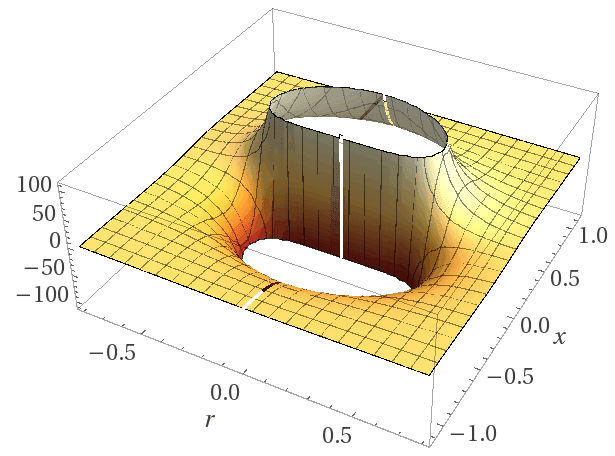
\includegraphics[width=\textwidth]{Pictures/Figure_primitivePlot.png}}
	  					\caption{\small $\hat{\varphi}\in C^\infty (\mathbb{R}^{n+1}\setminus{0})$ \\ in cylindrical coordinates $(x=x^0,r)$}
						\end{figure}		
					}
				%
	 	 	\end{column}
 	 \end{columns}






	


\end{frame}
\note[itemize]{
	\item
}
%-------------------------------------------------------------------------------------------------------------------------------------------------

%-------------------------------------------------------------------------------------------------------------------------------------------------
\begin{frame}[fragile]{HCMM for spheres \underline{(Transitive example)}}
	\begin{claimblock}[]
	Explicit HCMM for $SO(n+1) \circlearrowleft \left( S^{n}, \omega\right)$ \qquad($n$ even)
	\end{claimblock}
	\begin{columns}
	%
		\begin{column}{.4\linewidth}
			\begin{itemize}
				\item			Choose basis in $\mathfrak{so}(n)$:	
			\end{itemize}		
		\end{column}
		%
		\begin{column}{.65\linewidth}
	\[
	A_{a b} =(-)^{1+a+b}\left(
	\resizebox{.35\linewidth}{!} 
		{
			\bordermatrix{
								& &\scriptstyle a & & \scriptstyle b & \cr
               	& 0 &    & \cdots &  & 0 \cr
              \scriptstyle a	& 0  &  \cdots & 0 & 1 & 0\ \cr
               	& 0 &   & \cdots &  & 0\cr
              \scriptstyle b	& 0 & -1 & 0 & \cdots & 0 \cr
               	& 0  &   & \cdots &  & 0 }
		}
  \right)
  \]		
		\end{column}
	\end{columns}
	%
	\pause
	\vfill
	\begin{columns}
		\begin{column}{.4\linewidth}
			\begin{itemize}
				\item 			Fundamental vector fields:
			\end{itemize}
		\end{column}
		\begin{column}{.65\linewidth}
			\[v_{A_{a b}}=  (-1)^{1+a+b}\left(x^a \partial_b - x^b \partial_a\right)\]
		\end{column}	
	\end{columns}
	\pause
	\vfill
	\begin{columns}
		\begin{column}{1.05\linewidth}
			\begin{itemize}
				\item From the vanishing of $H^1(G),H^2(G)$ one gets:
				\begin{empheq}[box=\fbox]{align*}
					f_1 (A_{a b}) &= 
					- \iota(v_{F^1(A_{a b})}) \omega =
				\dfrac{1}{n-2}\sum_{k=0}^n \iota(v_{A_{k b}})\iota(v_{A_{k a}})\omega.				
					\\
					f_2(A_{a b} \wedge A_{c d}) &= 
					\dfrac{-1}{4}
						\sum_{k=1}^n	
					\left(
						\iota(v_{A_{k a} \wedge A_{k b} \wedge A_{c d}}) - 
						\iota(v_{A_{a b}\wedge A_{k c} \wedge A_{k d}})
					\right)\omega\\
					f_2(A_{j a} \wedge A_{j b}) &= \dfrac{-1}{n-2}
					\sum_{k=1}^n	
					\left(
						\iota(v_{A_{k a}\wedge A_{j b}\wedge A_{k j}})
					\right)\omega.
				\end{empheq}
				\pause
				\item 	Construction of $f_k$ with $k\geq 3$ can be addressed numerically.
			\end{itemize}
		\end{column}
	\end{columns}



\end{frame}
\note[itemize]{
	\item Recall that $\mathfrak{so}(n)$ is the Lie sub-algebra of $\mathfrak{gl}(n,\mathbb{R})$ consisting of all skew-symmetric square matrices. A basis can be constructed as follows:
\begin{equation}\label{eq:standard-basis}
	\mathcal{B}\coloneqq \big\lbrace 	A_{a b} = (-1)^{1+a+b} \left( E_{a b} - E_{b a}\right)
	\quad \vert \quad 1\leq a<b\leq n \big\rbrace
\end{equation}
where $E_{a b}$ is the matrix with all entries equal to zero and entry $(a,b)$ equal to one.
\item The fundamental vector field of $A_{a b}$ associated to the linear action of $SO(n)$ on $\mathbb{R}^n$ reads as follows:
\begin{displaymath}
	v_{A_{a b}}= \sum_{i,j}[A_{a b}]_{i j}x^j \partial_i  = (-1)^{1+a+b}\left(x^a \partial_b - x^b \partial_a\right)
\end{displaymath}
	\item from the vanishing of the first cohomology group of $(SO(n))$ one can give the action of $f_1$ and of $f_2$ (given on the only two subset of generators such that the image does not vanish)
	\item \textbf{$f_k$ for any $SO(n)$ and $k\geq 3$}:\\
	We know from Theorem \ref{thm:son-cohomology} that $H^3(\mathfrak{so}(n))$ never vanishes... how can we proceed? Tony drafted a code in Python. The repository is still private
}
%-------------------------------------------------------------------------------------------------------------------------------------------------


%
%
%
%%-------------------------------------------------------------------------------------------------------------------------------------------------
%\begin{frame}[fragile]{Results (Joint work with L. Ryvkin)}
%	\begin{thmblock}[\cite{Miti2019}]
%		Let $(M,\omega)$ multisymplectic, $G$ compact and $\vartheta: M \times G \to M$ preserves $\omega$. 
%		A HCMM exists if and only if
%		\begin{displaymath}
%			[\vartheta^\ast \omega - \pi^\ast \omega ] = 0 \in H_{dr}^{k+1}(M\times G)
%		\end{displaymath}
%	\end{thmblock}	
%
%\end{frame}
%\note[itemize]{

%	
%	\item 	
%	First 2 component of HCMM for $SO(n+1)$ on $S^{n}$ (Going higher can be set up as a computational problem - we have a sketch of code in Python -, the first 2 component are easier due to the vanishing of the first two CE cohomology group of $G$)
%}
%%-------------------------------------------------------------------------------------------------------------------------------------------------



%-------------------------------------------------------------------------------------------------------------------------------------------------

%---------------------------------------------------------------------------------------------------------------------------------------------------
%---------------------------------------------------------------------------------------------------------------------------------------------------
\thankyouslide
%-------------------------------------------------------------------------------------------------------------------------------------------------
%-------------------------------------------------------------------------------------------------------------------------------------------------








%------------------------------------------------------------------------------------------------
% APPENDIX
%------------------------------------------------------------------------------------------------
\appendix
\section{EXTRA}
%\sectionpage
\begin{frame}
	\begin{center}
	\Huge\emph{EXTRA}
	\end{center}
\end{frame}
\addtocounter{framenumber}{-1}

%------------------------------------------------------------------------------------------------
% Bibliography
%------------------------------------------------------------------------------------------------
% https://en.wikibooks.org/wiki/LaTeX/Bibliographies_with_biblatex_and_biber
\begin{frame}[t,allowframebreaks]{Extended Bibliography}
	%\nocite{*}
	\bibliographystyle{alpha}
	\bibliography{bibfile}
\end{frame}
%------------------------------------------------------------------------------------------------



%------------------------------------------------------------------------------------------------
%- HandOut Flag -----------------------------------------------------------------------------------------
\newif\ifHandout
	\Handouttrue  %uncomment for the printable version

%- D0cum3nt ----------------------------------------------------------------------------------------------
\documentclass[beamer,10pt]{standalone}
	%\setbeameroption{show notes}
	




%- Packages ----------------------------------------------------------------------------------------------
%\usepackage{verbatim}
\usepackage[mode=buildnew,subpreambles=true]{standalone}
\usepackage{import}
\usepackage{amsmath, amssymb}
\usepackage{tikz}
%\usetikzlibrary{arrows,shapes,calc}
%\usetikzlibrary{shapes.callouts}
\usepackage{tikz-cd}
\usepackage{hyperref}
\usepackage[english]{babel}
\usepackage{stackengine}

%--Beamer Style-----------------------------------------------------------------------------------------------
\usetheme{toninus}



%--Beamer Style-----------------------------------------------------------------------------------------------
\usetheme{toninus}





%---------------------------------------------------------------------------------------------------------------------------------------------------
%- D0cum3nt ----------------------------------------------------------------------------------------------------------------------------------
\begin{document}
%------------------------------------------------------------------------------------------------

%##################################################################################
\section{Background Material}
%##################################################################################

%------------------------------------------------------------------------------------------------
\begin{frame}[fragile]{MS geometry and classical field mechanics}\label{Frame:Ms-Field-Mechanics}
		Consider a smooth manifold $Y$,
		\begin{columns}
			\hfill
			\begin{column}{.5\linewidth}
				\emph{Multicotangent bundle} $\bigwedge = \bigwedge^n T^\ast Y$\\
				is naturally $n$-plectic
			\end{column}
			\begin{column}{.4\linewidth}
				\[
				\begin{tikzcd}
					\Lambda \ar[d,"\pi"'] & T \Lambda \ar[d,"T \pi"] \ar[l] \\
					Y								& T Y \ar[l]
				\end{tikzcd}	
				\]
			\end{column}
		\end{columns}
	\pause
	\begin{defblock}[Tautological $n$-form]
		$\theta \in \Omega^n(\Lambda)$ such that:
		\begin{displaymath}
		\begin{split}
			\left[ \iota_{u_1 \wedge \ldots \wedge u_n} \theta \right]_\eta 
			&= \iota_{(T \pi)_\ast u_1 \wedge \ldots \wedge (T \pi)_\ast u_n} \eta \\
			&= \iota_{u_1 \wedge \ldots \wedge u_n} \pi^\ast \eta 
			\qquad \qquad \forall \eta \in \Lambda \, , \: \forall u_i \in T_\eta \Lambda 		
		\end{split}
		\end{displaymath}
	\end{defblock}
	\vfill
	\begin{columns}
		\begin{column}{.6\linewidth}
			\begin{defblock}[Tautological (multisymplectic) (n+1)-form]
				$$\omega := d \theta$$
			\end{defblock}
		\end{column}
		\begin{column}{.4\linewidth}
		 	\begin{claimblock}$\omega$ is not degenerate.\end{claimblock}	
		\end{column}
	\end{columns}	
	\pause
	\begin{keywordblock}
		\begin{tabular}{|c|c|c|}
			\hline 
			point-particles mechanics & $\rightsquigarrow$ & classical fields mechanics \\
			%(finite discrete DOF) & & (finite dimensional continuous DOF) \\
			\hline 
			symplectic & $\rightsquigarrow$ & multisymplectic \\ 
			\hline 
			Observables (Poisson) algebra & $\rightsquigarrow$ & Observables $L-\infty$ algebra
			 \\ 
			\hline 
			Co-moment map & $\rightsquigarrow$ & Homotopy co-momentum map \\ 
			\hline 
		\end{tabular} 
	\end{keywordblock}

	
\end{frame}
\note[itemize]{
	\item This example is significant from the perspective of geometric classical field theory:
		\begin{displaymath}
			\frac{\text{classical mechanics}}{\text{symplectic geo.}} =
			\frac{\text{classical field mechanics}}{\text{multisymplectic geo.}}
		\end{displaymath}
	\item Multicotangent bundle is the \emph{Higher analogue} of the cotangent bundle.
	(but it is not yet the analogue of a \emph{phase space}.)
\item The multiphase space is the sub-bundle of $n$-forms vanishing when contracted with 2 vertical fields.
  	\item The reason why this sub-bundle has a particular role is that it can be proved to be isomorphic to a suitable dual of the first Jet bundle.
  	\item For further details see Gotay et al. \href{https://arxiv.org/abs/physics/9801019}{arXiv:physics/9801019}. For a pictorial representation of all the structures involved in the geometric mechanics of I order classical field theories see appendix, pag: \ref{frame:Gimmsy}.
}
%------------------------------------------------------------------------------------------------	
	
%------------------------------------------------------------------------------------------------
\begin{frame}{Special classes of smooth objects}\label{Frame:Classes-Multisymplectic-Objects}
  	\begin{columns}
		\begin{column}[t]{.42\linewidth}		
			\begin{defblock}[Hamiltonian v.f.]
				$\mathfrak{X}_{ham} =  \left\lbrace X \in  \mathfrak{X} \right\vert \left. \iota_x \omega \textrm{ exact}  \right\rbrace$ 			
			\end{defblock}
			\begin{defblock}[Multisymplectic v.f.]
				$\mathfrak{X}_{ms} =  \left\lbrace X \in  \mathfrak{X} \right\vert \left. \mathcal{L}_X \omega = 0  \right\rbrace$ 	
			\end{defblock}
		\end{column}
		\begin{column}[t]{.58\linewidth}		
			\begin{defblock}[Hamiltonian $(n$-$1)-$forms]
				\begin{displaymath}
					\Omega^{n-1}_{ham} 	:=
					\biggr\{ H \in  \Omega^{n-1} \; \left\vert \; 
					\stackanchor{$\exists X \in \mathfrak{X}_{ham}$}{: $d H = -\iota_X \omega$} \right\} 
			\end{displaymath}
			\end{defblock}		
		\end{column}
  	\end{columns}
  	%
  	\vspace{0.5em}
  	%
  	\onslide<2->{
  	\begin{columns}
		\begin{column}[t]{.5\linewidth}	
			\centering\emph{Global symmetries}
			\begin{defblock}[Multisymplectic (Lie group) action]
				$\Phi: G \circlearrowright (M, \omega)$ \emph{right action} s.t. \\
				$$\hat{\Phi}(g)_\ast \omega = \omega \quad \forall g \in G$$
			\end{defblock}
		\end{column}
		\begin{column}[t]{.5\linewidth}			
			\centering\emph{Infinitesimal symmetries}
			\begin{defblock}[Multisymplectic (Lie algebra) action]
				$V: \mathfrak{g} \rightarrow \mathfrak{X} (M)$ \emph{Lie algebra morphism} s.t. \\
				$$\mathcal{L}_{V_\xi} \omega = 0 \quad \forall \xi \in \mathfrak{g}$$	
			\end{defblock}
		\end{column}
  	\end{columns}
  	}
  	%
  	\onslide<3->{		
	  	\begin{asideblock}[Hierarchy of conserved quantities]%Shades of...
	  		\begin{table}[] % http://tablesgenerator.com/
			\begin{tabular}{lllll}
					& strictly conserved & & & $\mathcal{L}_X \alpha= 0$ \\
				$\alpha \in \Omega^\bullet$ & globally conserved & along $X \in \mathfrak{X}$ & $\Leftrightarrow$ & $\mathcal{L}_X \alpha\in B $ (exact) \\
				  & locally conserved  & & & $\mathcal{L}_X \alpha\in Z $ (closed)                                
			\end{tabular}
			\end{table}
	  	\end{asideblock}
  	}
  	
  \end{frame}
  \note[itemize]{
  	\item Exactly as it happens in symplectic geometry, fixing a smooth form $\omega$ on $M$ yields a criterion for classifying vector fields and differential forms.
  	\\(Pay attention to the sign convention in defining the Hamiltonian vector fields)
  	\item Also, we can naturally select a special class of symmetries (global and infinitesimal) which preserve the fixed multisymplectic form.
  	\item Aside, we can start to see that, in this setting, measurable quantities are not only smooth functions but also differential forms with degree greater then zero.
  	For such objects can be defined weaker notions of conservation along a flow.
  	\item The idea to consider forms of various degree as observables do not fall out of the sky. 
  		For instance in a string there will be two kind of measurable quantities: extensive observable (1-forms), like the density, and intensive observables (0-forms), like the tension. 
 		%\href{https://en.wikipedia.org/wiki/Intensive_and_extensive_properties#Intensive_properties}{(wiki link on this terminology)}
  	\item Starting from this observation we can define the space of all possible observables (see next slide).
  }
%---------------------------------------------------------------------------------------------------------------------------------------------------

\begin{frame}[fragile,shrink]{Unwrapping the \emph{higher Jacobi equations}}\label{Frame:unwapping-Jacobi}
\underline{Slogan:} \emph{Jacobi identity satisfied up to an higher coherent homotopy}
		%
		\vspace{1.5em}
		\begin{columns}[c]
			\hfill
			\begin{column}{0.5\linewidth}
				Higher Jacobi implies:
				\begin{itemize}  \setlength\itemsep{1em}
					\item Underlying chain-complex $(L,\mu_1)$ with differential $d=\mu_1$;
					\item \color{red} $\mu_2 = [\cdot,\cdot]$ is a chain map $L^{\otimes 2} \to L$;
					\item \color{green!20!black}$\mu_3=j(\cdot,\cdot,\cdot)$ is a chain homotopy 
						$\mu_2\circ\mu_2 \Rightarrow 0$;
						\\ i.e. between the usual Jacobiator ${[[\cdot,\cdot],\cdot]} \circ P_{\text{unsh}}$ and the $0$ map 
					\item \color{purple}higher analogues...	
					\\ e.g. $\mu_4$, is a second order chain-homotopy between the two chain homotopies  ${[j(\cdot,\cdot ,\cdot]),\cdot]}\circ P_{\text{unsh}}$ and ${j([\cdot , \cdot],\cdot,\cdot)}\circ P_{\text{unsh}}$
				\end{itemize}
			\end{column}
			\begin{column}{0.45\linewidth}
				\includestandalone[width=0.9\linewidth]{Pictures/Figure_Linfinity_diagram}
			\end{column}	
		\end{columns}	
		\vspace{1.5em}
		Notation: $P_{\text{unsh}}$ = sum on all the possibile unshuffled permutation.

\end{frame}
\note[itemize]{
  \item Regarding any $l_k$ as a tree with $k$ entries and 1 output, the $k$-th generalized Jacobi equation is produced summing all the possible way to obtain a $k+1$-ary tree by composing two other trees (not more then two!).
  \item Can be regarded as
  	\begin{displaymath}
  		\sum_{i+j = k} l_j \circ ( l_j \otimes \mathbb{I}) \circ P_{\text{unsh}}
  	\end{displaymath}
  	Where $P_{\text{unsh}} : L^{\otimes(k-1)} \rightarrow L^{\otimes(k-1)} $ is the $(i,j)$-unshuffolator.
  	\\(you consider only unshuffles to avoid the redundancies given by the fact that any $l_i$ has fixed symmetry.
  \item Examples of unshuffles: \\
  \begin{displaymath}
  \begin{split}
  	(12)(3)\quad(13)(2)\quad(23)(1)\\
  	(123)(4)\quad(234)(1)\quad(134)(2)\quad(124)(3)\\
  	(12)(34)\quad(23)(14)\quad(13)(24)\quad(14)(23)\quad(24)(13)
  \end{split}
  \end{displaymath}
	\item When regarding the L$\infty$ structure as a chain complex with homotopies you get a neat intepretation of the Jacobi identity at the price that \emph{graded skew-symmetry} definition is more obscure than in the presentation with graded vector spaces.
}
%------------------------------------------------------------------------------------------------



%------------------------------------------------------------------------------------------------

% Frame inspired by Leonid: passing from moment maps to comoment maps
\begin{frame}[fragile]{Reminder: Moment maps in symplectic geometry}
	Let $(M,\omega)$ be a symplectic manifold, $\vartheta: G\times M \to M$ a Lie group action preserving $\omega$ and $v:\mathfrak{g}\to \mathfrak{X}(M)$ the corresponding infinitesimal action
	%
		\begin{defblock}[Moment map pertaining to $\vartheta$]
			Smooth map $ \mu: M \to \mathfrak{g}^\ast$ such that: \stackunder{$d \langle\mu , \xi \rangle = \iota_{v_\xi}\omega \scriptstyle\quad \forall \xi \in \mathfrak{g}$}{$f (\vartheta_g(x)) = Ad^\ast_g (f(x)) \scriptstyle\quad \forall g \in G, x \in M$}
		\end{defblock}
	%
	\vfill
	\emph{... from a dual perspective (assuming $G$ connected) ...}
			\begin{defblock}[Comoment map pertaining to $v$]
				\begin{columns}
					\begin{column}{.5\linewidth}	
			Lie algebra morphism \qquad $ f: \mathfrak{g} \to C^\infty(M) $
			\\
			such that \qquad $ d~f (x) = -\iota_{v_x} \omega \qquad \forall x \in \mathfrak{g}~.$
					\end{column}
					\begin{column}{.4\linewidth}	
						\begin{displaymath}
							\begin{tikzcd}
								& C^{\infty}(M,\omega) \ar[d]
								\\
								\mathfrak{g} \ar[ur,dashed,"(f)"]\ar[r,"v"']& \mathfrak{X}(M)
							\end{tikzcd}	
						\end{displaymath}
					\end{column}
				\end{columns}
		\end{defblock}		
	%
	\vfill
	\emph{... a tool encoding conserved quantities ...}
	\begin{propblock}[Noether Theorem]
		\small Fixed $H\in C^\infty_{\text{Ham}}(M)$ ($\mathfrak{g}$-invariant) ,
				$$\mathcal{L}_{v_H} f(x) = 0 \qquad \forall x \in \mathfrak{g}$$
	\end{propblock}
\end{frame}
%\note[itemize]{
%	\item comoment map is a Lie algebra morphism projecting to $v$. (Triangle diagram in Lie algebra category).
%}



%------------------------------------------------------------------------------------------------
\begin{frame}{Geometry of symmetries}\label{frame:geometrysymmetries}
	Basic mechanical structures are encoded in geometry. but there is another complementary geometrical property that's natural in physics: symmetry!
	\begin{alertblock}{Upshot}
		Continous symmetries are described by actions of a Lie group on $M$.
	\end{alertblock}
	\begin{block}{Noether}
		Presence of symmetries $\quad \Rightarrow \quad$ existence of conserved quantities.
	\end{block}	
	\begin{block}{Key concept:}
		Noether current are encoded in a \emph{moment map}  $\mu :M \rightarrow \mathfrak{g}^*$ (the dual of the comoment map $f$. 
	\end{block}
  \begin{columns}[T]
   	\begin{column}{.6\textwidth}
			\begin{block}{Symplectic reduction:}
			\begin{itemize}
				\item System dynamics should be restricted to level set of conserved observables in order to efficiently store dynamical properties.
				\item Under certain assumptions, $\mu^{-1}( 0 )/G$ is a symplectic manifold with an "induced" symplectic structure.
			\end{itemize}
			\end{block}
    \end{column}
    \begin{column}{.4\textwidth}	
			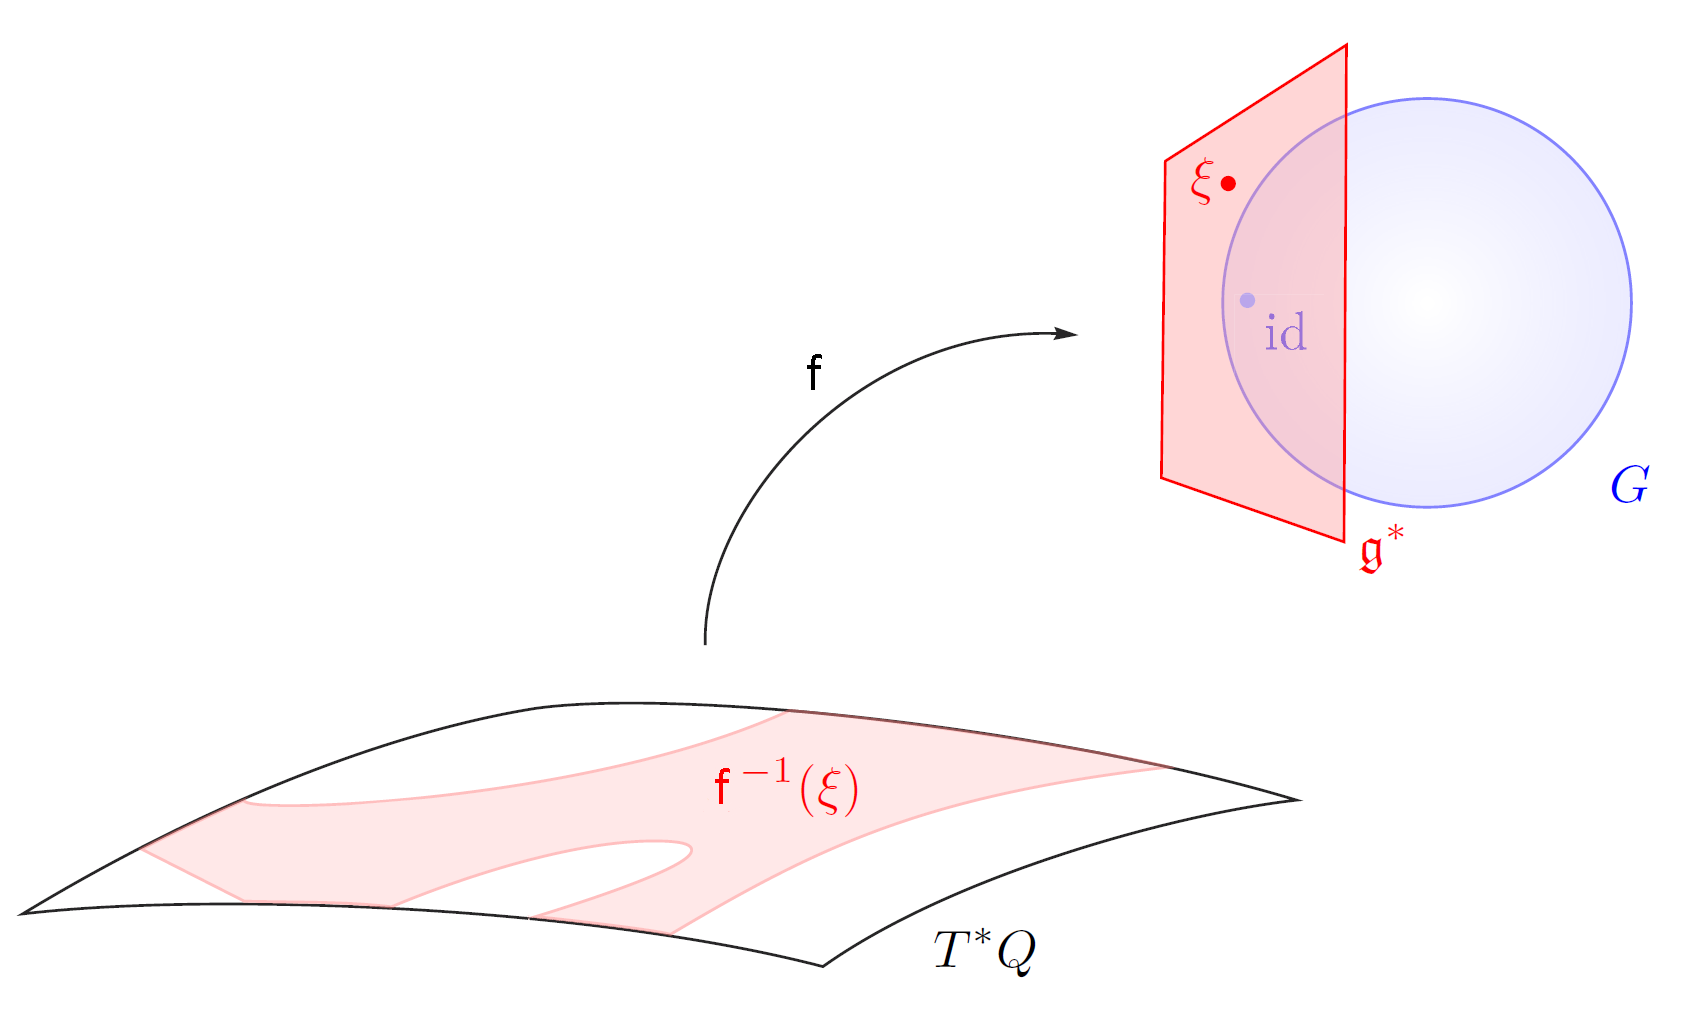
\includegraphics[width=\textwidth]{Pictures/Reduction} 
  	\end{column}
	\end{columns}			
\end{frame}
%------------------------------------------------------------------------------------------------

%##################################################################################
\section{Work Done with Leonid}
%##################################################################################
%-------------------------------------------------------------------------------------------------------------------------------------------------
\begin{frame}[fragile]{Cohomological obstructions for compact groups}\label{frame:cohomologicalproposition}
	Let $\vartheta:G\times M\to M$ be a compact Lie group acting on a pre-multisymplectic manifold, preserving the pre-multisymplectic form $\omega$. 
	%
	\begin{propblock}
		[ $\exists$ (HCMM) $ 
			~\Leftrightarrow~ 
			\lbrack\vartheta^*\omega-\pi^*\omega\rbrack=0\in H^{n+1}(G\times M)$]
		Based on the sequence of isomorphisms:
		\begin{center}
			\begin{tikzcd}
	 			\Omega^\bullet(M,\vartheta) \ar[d,"\vartheta^\ast-\pi^\ast"] &\quad
				 & H_\text{dR}(M) \ar[d,"\vartheta^\ast-\pi^\ast"]  
				 & \lbrack \omega \rbrack \ar[d,mapsto]
				 \\ 
				 \Omega^\bullet(G\times M, r\times id) \ar["\cong",leftrightarrow]{d} &\quad
				 & H_\text{dR}(G\times M) \ar[leftrightarrow,"\cong"]{d}[swap]{\text{\tiny (K\"unneth)}} 
				 & \lbrack \vartheta^\ast \omega - \pi^\ast \omega \rbrack \ar[ddd,mapsto]
				 \\ 
				 \Omega^\bullet(G,r) \otimes \Omega^\bullet(M) \ar["\cong",leftrightarrow]{d}[swap]{} &\quad
				 & H_\text{dR}(G) \otimes  H_\text{dR}(M) \ar[d,"\cong",leftrightarrow]
				 \\ 
				 \Lambda^\bullet \mathfrak{g}^* \otimes \Omega^\bullet(M)\ar["\cong",leftrightarrow]{d} &\quad
				 & H_\text{CE}(\mathfrak{g}) \otimes  H_\text{dR}(M) 
				 \ar["\cong",leftrightarrow]{d} & 
				 \\
				 C_\mathfrak{g}^\bullet \oplus ( \mathbb{R}\otimes \Omega^\bullet(M))&\quad 
				 & H(C_\mathfrak{g}^\bullet)\oplus H_\text{dR}(M)
				 & \lbrack \tilde{\omega}\rbrack
			\end{tikzcd}
		\end{center}						
	\end{propblock}
\end{frame}
%-------------------------------------------------------------------------------------------------------------------------------------------------

 %------------------------------------------------------------------------------------------------
  \begin{frame}[fragile,t]{Chevalley-Eilenberg Complex}\label{frame:CE-complex}
  	Consider $\mathfrak{g}$, Lie Algebra.
  	\begin{defblock}[Eilenberg-Chevalley Complex]
  		Chain Complex
			\begin{center}
				\begin{tikzcd}[column sep= small,row sep=0.25ex]
					\ldots \ar[r,"\partial"] & \wedge^k \mathfrak{g} \ar[r,"\partial"] & 
					\wedge^{k-1} \mathfrak{g} \ar[r,"\partial"] & \ldots
			\end{tikzcd}	
			\end{center}
			with chain group
			\begin{displaymath}
				C^k := \wedge^k \mathfrak{g} \equiv 
				\big\{ c : \mathfrak{g}^\ast\times\ldots\mathfrak{g}^\ast \to \mathbb{R}\:\big\vert\, \textrm{alternating, k-linear} \big\}
			\end{displaymath}
			and boundary operator defined as
			$\partial \equiv \partial^k :  \Lambda^{k} {\mathfrak g} \to \Lambda^{k-1} {\mathfrak g}$  via
			$$
				\partial (\xi_1 \wedge \xi_2 \wedge \dots \wedge \xi_k) := \sum_{1\leq i< j \leq k} (-1)^{i+j}\, [\xi_i, \xi_j] \wedge \xi_1 \wedge \dots {\hat \xi}_i \wedge \dots \wedge {\hat \xi}_j \wedge \dots \xi_k
			$$
			where $\hat{}$ denoting deletion and with $\partial_0 = 0$.
  	\end{defblock}
		\begin{claimblock}
			$$\partial^2 = 0$$
		\end{claimblock}		
  \end{frame}
 % \note{}
%------------------------------------------------------------------------------------------------


%------------------------------------------------------------------------------------------------
\end{document}

%------------------------------------------------------------------------------------------------



\end{document}

